\documentclass[11pt, a5paper, parskip=half-, DIV=12]{scrartcl}

\usepackage{../endeavour}
\usepackage{../endeavour_book}

\version{0.1}

\begin{document}
% Colour Cover
\thispagestyle{plain}
\AddToShipoutPictureBG{
\begin{tikzpicture}[remember picture, overlay]
	\node () at (current page.center) {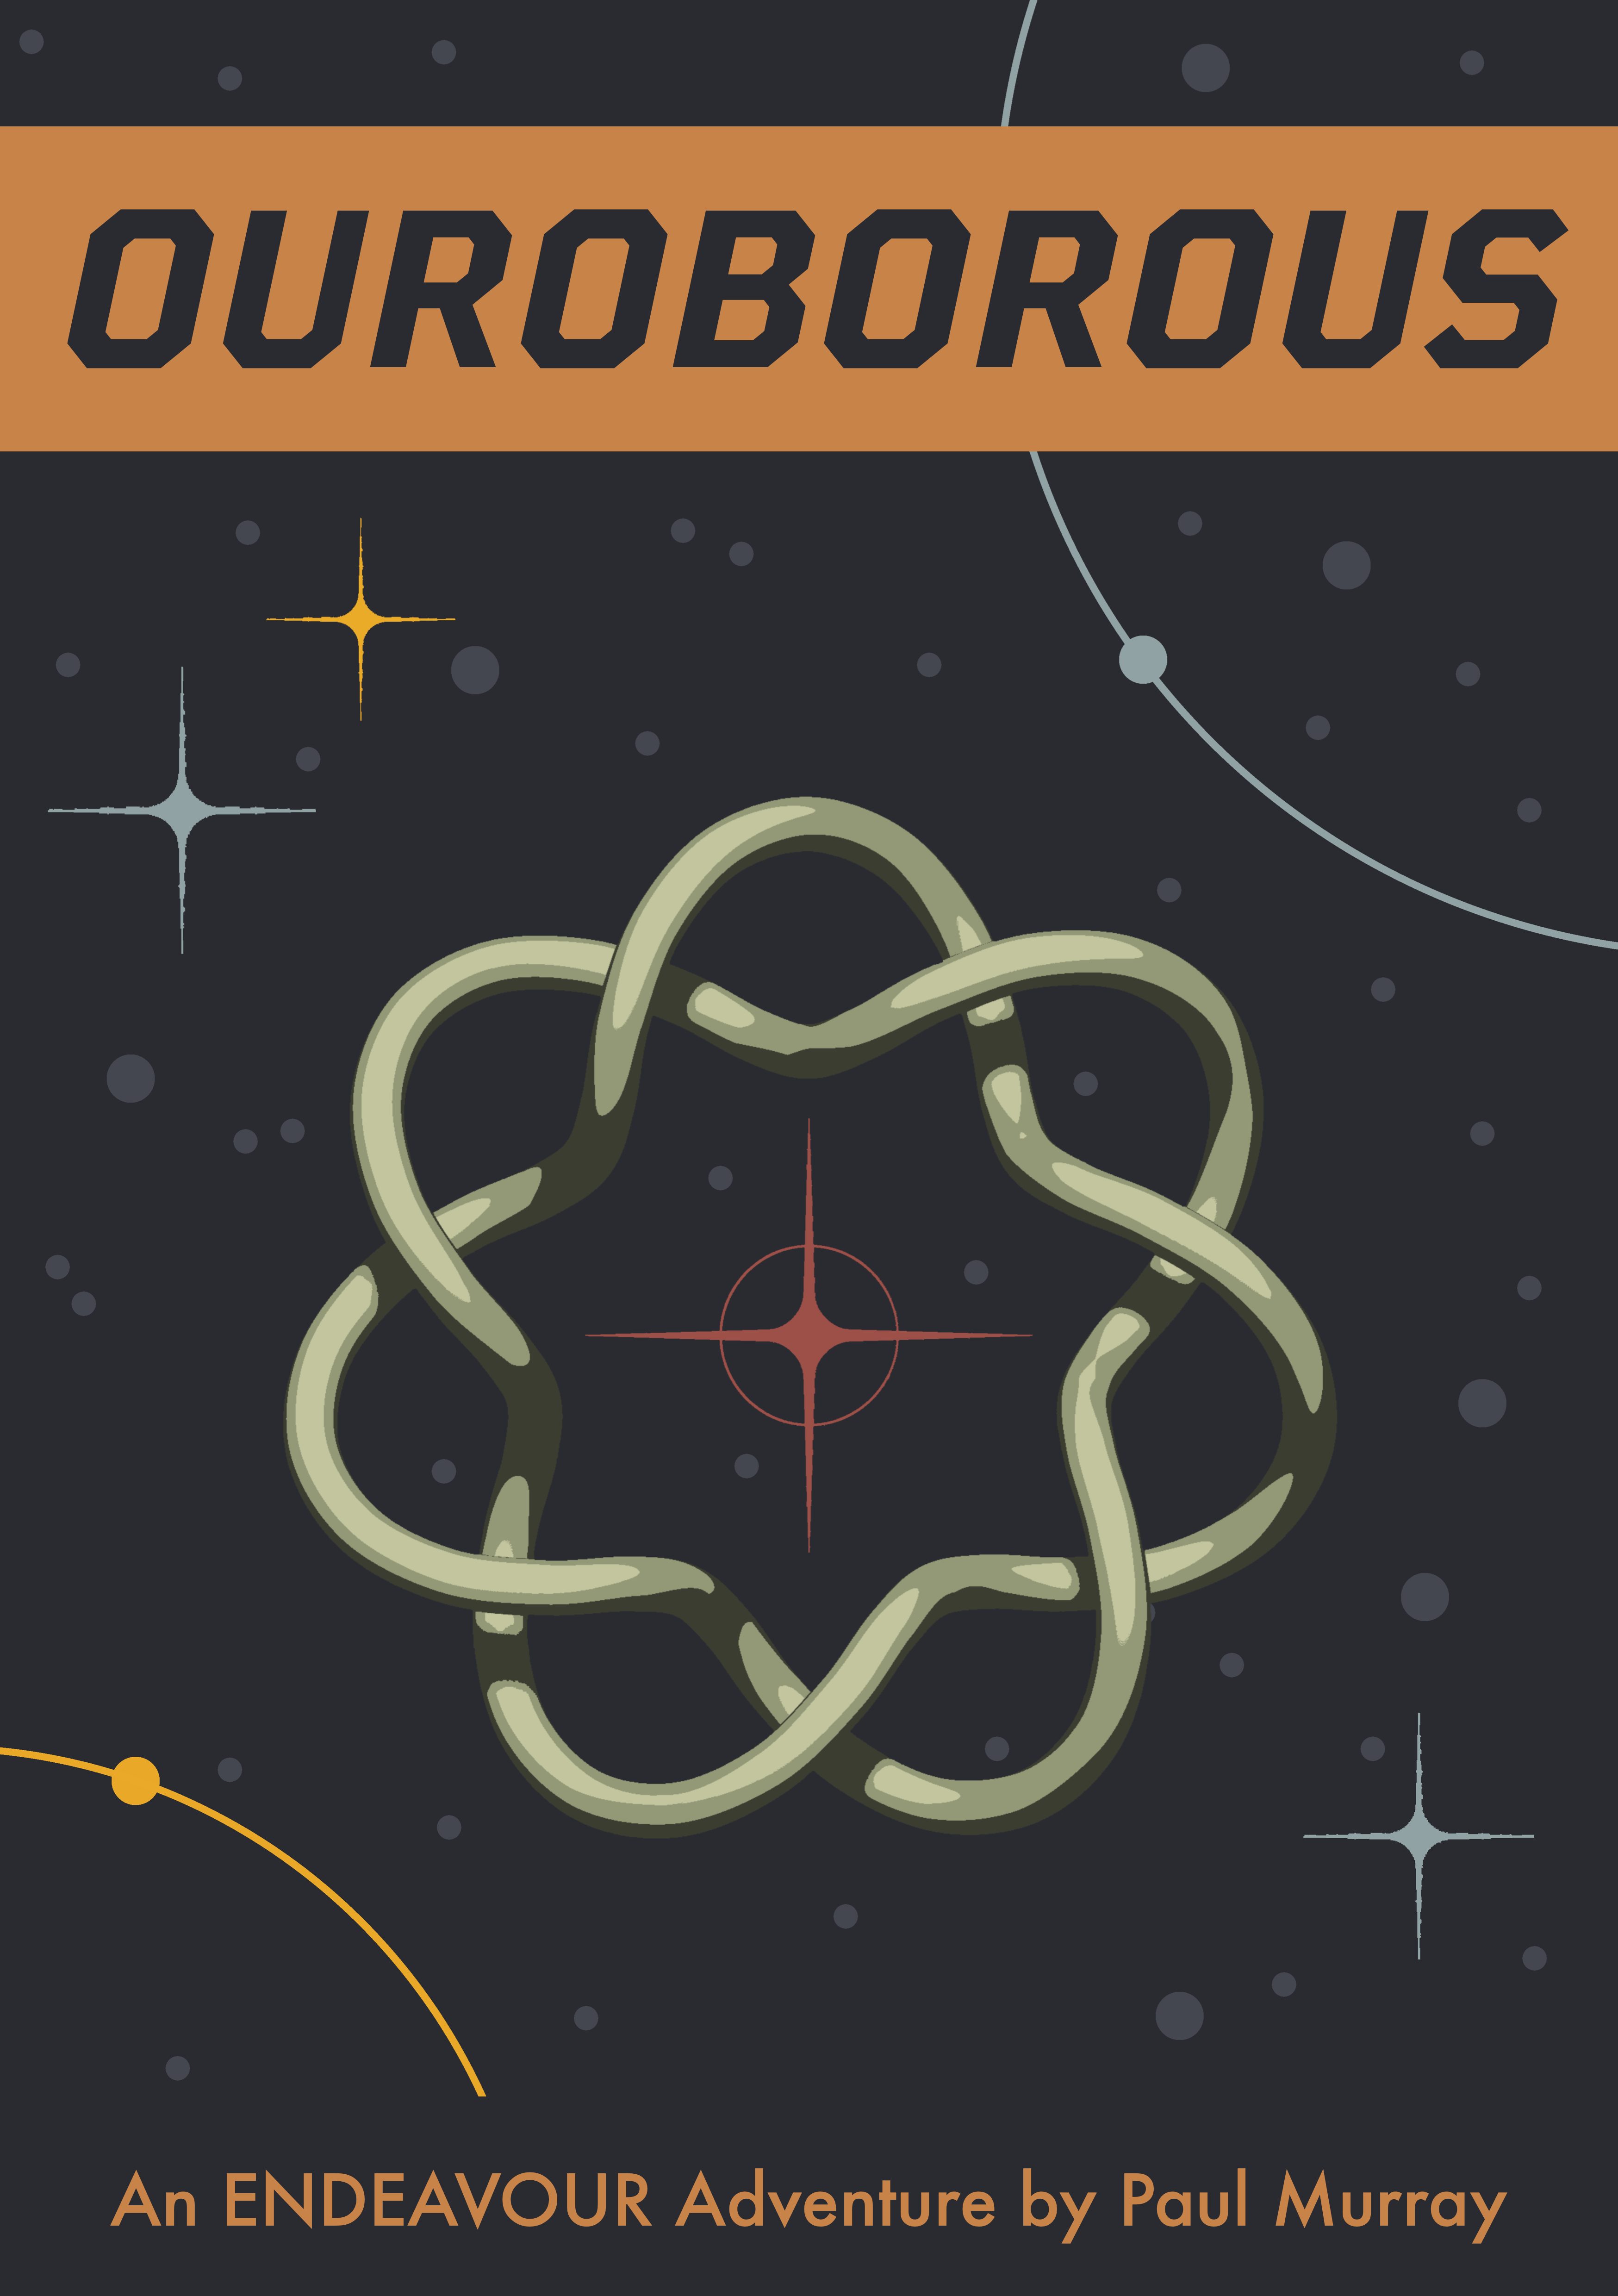
\includegraphics[width=\pagewidth, height=\pageheight]{Images/ouroborous_cover.png}};
\end{tikzpicture}
}
{
\colorlet{headfootcolor}{LCARS_ORANGE}
\phantom{a}

\newpage
}

\ClearShipoutPicture
\AddToShipoutPictureBG{
	\begin{tikzpicture}[remember picture, overlay]
	\pic () at (current page.center) {starfield};
		\node[endeavour_box, minimum width=12.6cm, minimum height=18.8 cm] at (current page.center) {};
	\end{tikzpicture}
}

\setcounter{page}{1}
\setmainfont{TeX Gyre Schola}
\normalsize
\raggedright

\section*{Ouroborous}
\textit{\textbf{Captain's Log:} Deep space monitoring stations have recently detected a series of subspace field events in the vicinity of Station E-59. Superficially similar to the emanations of a faster-than-light drive, the phenomena are far more powerful than what any known device is capable of producing.}

\textit{Station E-59 was recently acquired by Ophidian Research, \\a newly incorporated \textemdash{} and rather secretive \textemdash{} private company. They have declined to respond to requests for information about their activities. The Endeavour has been dispatched by ICF command to investigate.}

\subsection*{Arrival}
When you arrive at Station E-59, you find that the station is at the heart of a construction project.  Ophidian Research is building a massive \textbf{Outer Ring} around the original station. Together, the the two structures are known as \textbf{Ouroborous}.

After an extended delay, \textbf{Patala} responds to your hails. She is an Ophidian, a species of reptilian humanoids only rarely encountered by the Interstellar Confederation. She demands that you identify yourself and state your business here.

\subsubsection*{Challenge Name}
\begin{itemize}
	\item \textit{Will you try to enlist Patala's help in your investigation?} \textbf{Leadership \& Negotiation} vs. \textbf{Patala}. This is a \textit{Fraught} challenge \textemdash{} Patala is suspicious that you might try to shut down her operation. If you prevail, gain a 1d8 Advantage die on all challenges vs. Subspace Field Event.
	\item \textit{Or will you try to convince Patala to allow you to access Ouroborous without explaining why you are here?} \textbf{Strategy \& Tactics} vs. \textbf{Patala}. If you prevail, gain a 1d8 Advantage die on all challenges vs. Jyotika.  
\end{itemize}

\newpage

\subsection*{Trials}
\subsubsection*{Malicious Compliance}
After a lengthy reception, \textbf{Jyotika} guides you on a tour of Ouroborous. He describes every facet of the operation in excruciating detail. \textit{Can you distinguish between useful information and irrelevant details in what he tells you?} \textbf{Operations \& Engineering} vs. \textbf{Jyotika}.

\subsubsection*{The Perfect Storm}
Many of the junior Ophidian researchers become agitated when they detect evidence of precursors to another subspace field event. All signs indicate that this will be the biggest such event that they have ever observed. \textit{Can you discern why this is a cause of agitation rather than of excitement?} \textbf{Science \& Medicine} vs. \textbf{Subspace Field Event}.

\subsubsection*{Great Expectations}
Surasa, a mid-level Ophidian researcher, arranges a meeting with the inspection team. He explains that he is pregnant and begs you to help him find a way to leave Ouroborous before the next subspace field event occurs. \textit{Can you convince Patala to allow Surasa to leave Ouroborous without revealing his condition?} \textbf{Strategy \& Tactics} vs. \textbf{Patala}.

\subsection*{Crisis}

\begin{itemize}
	\item \textit{Will you try to disrupt the predicted subspace field event?} \textbf{Threats:} The inspection team's security detail is killed by Ophidian zealots. The Endeavour is recalled after Patala lodges a formal protest with ICF command. A rift in space appears at the epicenter of the phenomena.
	\item \textit{Or will you try to withdraw to a safe distance to observe the phenomenon?} \textbf{Threats:} Surasa's babies are killed. Any Ophidians on Ouroborous are sterilized.  The Endeavour's faster-than-light drive is disabled. 
\end{itemize}

\newpage

\subsection*{Characters}
\begin{description}
	\item[Patala (d10):] Station Director (d10), Meticulous (d8), Determined (d8), Administrator (d8 \textit{Sensitive}).
	\item[Jyotika (d10):] Senior Researcher (d10), Scientist (d10), Experienced (d8), Mystic (d8), Zealot (d8).
%	\item[Surasa (d8):] Mid-level Researcher (d8), Artist (d8), Scientist (d8), Desperate (d8), Insightful (d6).
	\item[Subspace Field Event (d12):] Unfamiliar (d10), Enormous (d10 \textit{Grueling}), Powerful (d10 \textit{Dangerous}). \textbf{\textsc{Amplified}} (Roll all dice twice and use the larger result).
\end{description}

\subsection*{Places}
\begin{description}
	\item[Station E-59:] An old space station.
	Extensively refurbished,
	it is home to over one thousand Ophidians.
%	every surface is covered with artwork.
	\item[Outer Ring:] An irregular twisting helix that surrounds Station E-59. It is unfinished and partially evacuated.
	The Outer Ring is entirely covered by intricate artwork.
	%Construction crews race to complete the structure.
%	\item[Place Name:] Brief description.
\end{description}

\subsection*{Mysteries}
\begin{description}
	\item[The subspace field events are natural phenomena.] \phantom{} \\ The purpose of Ouroborous is to amplify preexisting subspace field events. The Ophidians believe that studying these phenomena will help them understand the ``fundamental nature of reality''. \textit{Why are the Ophidians so secretive about what they are trying to do here? Who is providing the funding to support their research?}
	\item[There are no children on Ouroborous.] \phantom{a} \\The subspace field events are fatal to juvenile Ophidians. Most of the scientists and artisans on Ouroborous are well past reproductive age. \textit{How are mature Ophidians affected by the subspace field event? How did they discover the threat posed by the phenomena?}
%	\item[The Outer Ring is covered in intricate artwork.] \phantom{a} \\ The majority of the Ophidians on Ouroborous are artisans who are entirely dedicated to decorating the Outer Ring. The artwork does not appear to have any practical purpose. \textit{Why are the Ophidians so focused on their artistic endeavors? What does the art represent?}
\end{description}

\newpage

\section*{Acknowlegements}
Much of the look and feel of \ENDEAVOUR{} is derived from its art, all of which was created by \textbf{svekloid}. This art was assembled from multiple collections available online at \href{http://shutterstock.com}{shutterstock.com} and then modified by Michael Purcell.  

\subsection*{Playtesters} \label{subsection:playtesters}
The following people helped to create \ENDEAVOUR{} by playing early versions of the game and providing invaluable feedback.\vspace{-1.75ex}
\begin{multicols}{2}
\begin{itemize}[noitemsep]
  \item Keydan Bruce
  \item Dannielle Harden
  \item Andrew Hellyer
%  \item Sarah Hewat
%  \item Scott Joblin
%  \item Sen-Foong Lim
  \item David McKenzie
%  \item Holly Moore
  \item Paul Murray
%  \item David Purcell
%  \item Heidi Purcell
  \item Kira Purcell
  \item Luke Purcell
  \item Meagan Purcell
%  \item Steve Purcell
%  \item Jason Stark
  \item Jo Stephenson
%  \item Pieter Vismans
  \item Brett Witty
  \item Bevis Worcester
  \item Evan Worcester
\end{itemize}
\end{multicols}

\subsection*{Design Tools} \label{subsection:design-tools}
The following tools were used to create this document:
\begin{description}[font=\normalfont\textbullet\space, noitemsep, topsep=-1ex]
	\item[LuaLaTeX:] Typesetting and layout.
	\item[TikZ:] Diagrams and art.
\end{description}
\vspace{1ex}
The fonts used are {\setmainfont{TT Mussels-BoldItalic} TT~Mussels~Bold~Italic},  \textsf{Futura}, and TeX~Gyre~Schola (cf. Century Schoolbook).

\vfill

\begin{tabular}{@{}m{7.775cm}@{\hspace*{0.375cm}}>{\centering\arraybackslash}m{2.6cm}@{}}
\textbf{Contact:} \href{mailto:endeavour.ttrpg@gmail.com}{endeavour.ttrpg@gmail.com}\newline \phantom{This is a test, only a test.} \newline \footnotesize{For use with the \textsc{Paragon} system, ©2020\newline \textbf{John Harper \& Sean Nittner}. \href{http://agon-rpg.com}{AGON-RPG.com}} & \includegraphics[scale=0.175]{Images/paragon_logo_mark.png} \\[5ex]
\footnotesize{This work is licensed under a Creative Commons \newline ``Attribution-ShareAlike 4.0 International'' license.} & \Huge{\doclicenseIcon}
\end{tabular}

\newpage

\thispagestyle{empty}

\tikzset{starfield/.pic={
	\node () at (current page.center) {
\includegraphics[width=\pagewidth, height=\pageheight]{Images/starfield.png}};
}}

\ClearShipoutPicture
\AddToShipoutPictureBG{
	\begin{tikzpicture}[remember picture, overlay]
	\pic () at (current page.center) {starfield};
	\end{tikzpicture}
}

\phantom{a}

\end{document}